\chapter{The Quest for a Quantum Computer}
Before delving into the question of how we might build a quantum computer, it is worth taking a step
back and exploring the question of what brought us as a scientific community to the point where
it is seen as a priority to build one. The answer to that requires us to delve briefly into
the world of computational complexity theory, and to examine what it means to solve problems "efficiently".
Although the genesis of computation can be traced back to pioneering works by people such as Charles Babbage
and Ada Lovelace in the early 1800's~\cite{Bowden:1953:FTS:1102044}, it was not until the early 1900's that
machines we might recognize as computers were constructed. Based on delicate vacuum tubes, mechanical relays
and often taking up full rooms, their inherent fragility and bugginess posed formidable obstacles to scaling.
It was not until the mid-1900's that the field took off with two pivotal discoveries. The first
was the construction of the first transistor in 1947, credited to Bardeen, Brittain and Schockley and for which
they were awarded the Nobel prize in 1956~\cite{nobel1956}. This was followed by the creation of integrated circuits by Jack Kilby
in 1959, for which he was awarded the Nobel prize in the year 2000~\cite{nobel2000}. With these two inventions, a remarkable
surge in computational power occurred. This surge is embodied in Moore's law, which described an annual
doubling in the number of transistors that it would be possible to fit on a single integrated circuit~\cite{4785860}.
And with this doubling came an exponential growth in the computation power that we had available to us.

Along with this growth came an obvious question. What exactly can these computers do? What sorts of
problems will we be able to solve with our ever-growing bundle of transistors? To do this, we need to
think about how many steps it takes to run various algorithms. Take for example the question of looking
for a single item $x_T$, in a list $L = \{x_0, x_1, ..., x_n\}$ with $n$ items in it. Assuming the list
is in an unknown order, to find the location of the item $x_T$, we need to look at each item in the list
in turn. If the length of the list were doubled to $2n$ items, it would take twice as many comparisons to
look through the list. Tripled would be three times. The amount of time it takes to find an item in the
list is \emph{linear} in the length of the list. We can write this mathematically using big$\mathcal{O}$
notation: searching for an item in a list is $\mathcal{O}(n)$.

What about a slightly more complicated problem. What if we want to check whether any item $x_i$ appears
in the list twice? To run this algorithm, we can run the above algorithm for each item in the list, setting the
target to $x_T = x_0$, then $x_T = x_1$ and so forth, and checking whether we find the item two or more
times. So for $n$ items in the list, we run through the list $n$ times, so the number of steps to run
the algorithm scales as $\mathcal{O}(n^2)$. That is, if the length of the list is doubled, it takes
four times as long, so the scaling is \emph{quadratic}.
In this way, we can classify algorithms into various complexity classes. For example, sorting a list
of $n$ items is in the best case $\mathcal{O}(n \log(n))$. Solving the travelling salesman problem (TSP) is
$\mathcal{O}(n^2 2^n)$. More generally, we can group problems into those that have at worst a polynomial
complexity, i.e. $\mathcal{O}\left(f(n)\right)$ where $f(n)$ is a polynomial. These problems are
in the complexity class \cc{P} (for polynomial), and are said to be \textbf{efficiently} computable.
Those problems that have a difficulty that grows faster than a polynomial in the size of the problem,
for example, problems whose complexity grows exponentially, are said to be inefficient to compute.

Of course, you might say, well what sort of operations do we allow our computers to do in a single step?
If I say that my computer can solve the TSP in a single step, then the complexity reduces trivially to
$\mathcal{O}(1)$. The answer is not so trivial --- it is limited by the laws of physics. What sorts
of computation do they allow? To answer this question, Alan Turing and Alonzo Church came up with the notion of
the Turing Machine, a universal model for a computational device, and with it stated the Church-Turing
hypothesis:

\begin{displayquote}[\cite{turingthesis}]
  "a function is effectively calculable if its values can be found by some purely mechanical process".
  We may take this literally, understanding that by a purely mechanical process one which could be carried out by a machine.
\end{displayquote}

To paraphrase, this stated that anything a Turing machine could do, a computer could do too, and anything
it \emph{can't} do, no computer can. It wasn't long before this was extended to the strong Church-Turing
hypothesis, which states \textquote[\cite{kaye2007an}]{A probabilistic Turing machine can efficiently simulate any
realistic model of computation}.
\footnote{In fact, we have to make an addition to the class of algorithms that a Turing machine can run efficiently
 due to the discovery of probabilistic algorithms, which can solve some problems with $> 2/3$ chance in
 polynomial time. By running these algorithms repeatedly, we can solve problems to within an arbitrarily small
 error $\epsilon$. This class of efficiently computable functions is called bounded-error probabilistic polynomial (\cc{BPP}).}
Note the addition of the term \textbf{efficiently}. This implies that for any
operation we could add to any hypothetical computer, we can get at most a polynomial speedup. Since
a polynomial $P(n)$ divided by another polynomial $Q(n)$ is still a polynomial, and anything that grows faster
than a polynomial $E(n)$ divided by a polynomial $Q(n)$ still grows faster than a polynomial, we have
a universal definition for problems that are efficient to solve and those that aren't.
\footnote{Of course, since we're continually coming up with better algorithms to solve hard problems,
the set of algorithms that are efficient to solve seems to keep growing!}


\begin{figure}
  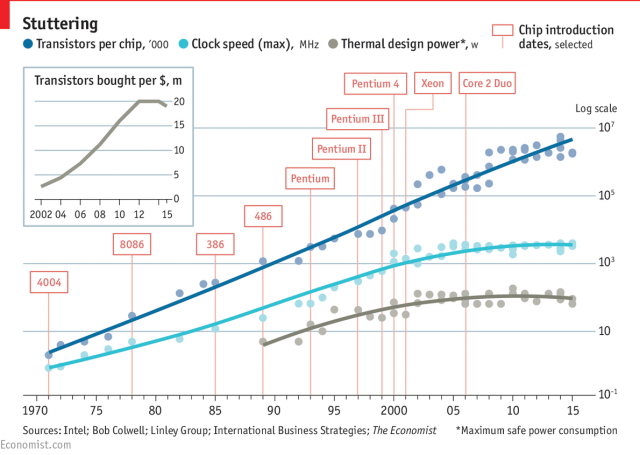
\includegraphics[width=0.7\linewidth]{MooresLaw}
  \caption[Moore's Law and the end of exponential scaling]
  {Graph of the number of transistors per chip, their clock speed, and their
  thermal design power plotted on a log scale against time. Although the number of transistors per chip
  continues to grow exponentially, the clock speed and power per chip have plateaued in the early 2000s.
  Reproduced with permission from~\cite{cross_2016}.}
  \label{fig:mooreslaw}
\end{figure}

So we've established what sorts of problems a computer can solve efficiently, and we've also noted the
exponential growth in the number of transistors on a chip. As long as both of these facts remain true, we
should only have to wait a few years before our computers become twice as powerful and problems that were
previously intractable fall within our grasp. Unfortunately, any exponential scaling must eventually fail,
and so it was for ICs for two key reasons: power and transistor size. As we made our transistors smaller,
we stopped seeing a concomitant efficiency increase, and all of a sudden, the power density of our ICs
became a limiting factor. To halt this increase, we had to reduce power dissipation, and the
only way we saw how was by capping the speed of our computers, which we can see in figure~\ref{fig:mooreslaw}
has plateaued since the early 2000s. Moreover, the smaller our transistors became, the more costly they became
to make. Even Moore's law, which has stubbornly held past the expectations of most scientists, must eventually
end as we bump up against the sizes of atoms. It seems unlikely that there is much room below Samsung's
recently announced \SI{3}{\nano\meter} node, so if we want to bring more problems into the fold of the
possible, it seems like the strong Church-Turing hypothesis must give.

It was in this context that Feynmann gave his seminal address, noting that as far as we can tell, simulating
quantum systems falls outside of the set of problems that are efficient on classical computers\cite{Feynman1982}.
However, as long as we can manipulate quantum systems, we should also be able to set up a "quantum
simulator" to see how a quantum system behaves. If this turned out to be the case, then the strong
Church-Turing hypothesis would be violated!\footnote{Despite this violation, as far as we know the original
Church-Turing hypothesis still holds. No previously uncomputable function became computable with the addition
of quantum physics.} Here was nature efficiently simulating a system that as far as we know, a Turing machine
can't. It was David Deutsch who in 1985 formalized the idea of a quantum Turing machine\cite{doi:10.1098/rspa.1985.0070},
and laid out the Deutsch-Church-Turing hypothesis, which as far as we know holds to this day:

\begin{displayquote}
  A quantum Turing machine can efficiently simulate any realistic model of computation.
\end{displayquote}

\begin{figure}
  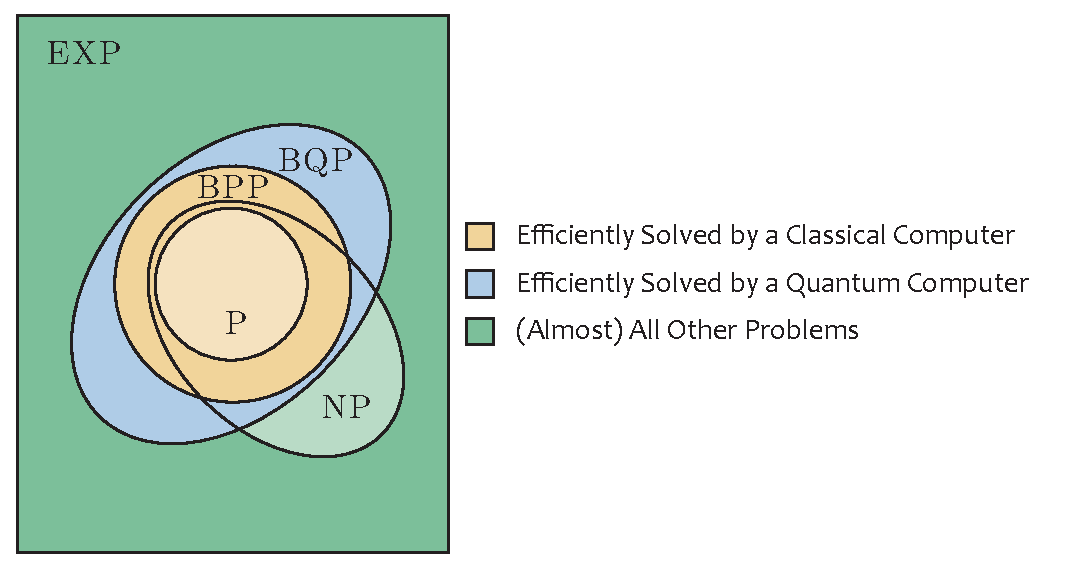
\includegraphics[width=0.85\linewidth]{ComplexityClasses}
  \caption[Relationship between various complexity classes]
  {Relationship between the various complexity classes that we've discussed. The class
  \cc{BPP} includes all problems that a classical computer can solve efficiently (including
  everything that can be calculated in polynomial time). \cc{BQP} are all problems a quantum computer can
  solve efficiently (which includes everything a classical computer can do). Finally, problems that scale exponentially
  with input size, labelled \cc{EXP}, are (almost) all other problems that are computable. The class
  \cc{NP} is also included on this figure as it is one that often comes up in the context of complexity,
  if for no other reason than to emphasize that a quantum computer \emph{cannot} solve all problems in
  this class.}
  \label{fig:complexity}
\end{figure}

With that, we finally define the class of problems that we might be able to solve efficiently if we
can build a quantum computer --- Bounded-Error Quantum Polynomial-Time or \cc{BQP}. As far as we know,
this class includes interesting problems that a classical computer could not efficiently solve. Problems
such as Shor's algorithm for prime factorization\cite{Shor} or estimating the ground state of molecules with
the Variational Quantum Eigensolver algorithm\cite{ncomms5213} have no known efficient classical algorithm
but could profoundly impact society if they are solvable. It is the promise of solutions to these problems
that drive the search for a quantum computer; however, the challenges of realizing one remain formidable. To close
out our discussion of complexity classes, I've summarized the relationship between complexity classes in
figure~\ref{fig:complexity}. To emphasize this point, note that although \cc{BQP} is larger than \cc{P}
or \cc{BPP}, it certainly does not enclose all problems, especially those in \cc{EXP}. Although a
quantum computer may offer an exponential speedup on a subset of algorithms, it will not give us an exponential
speedup in the general case.

The remainder of this chapter aims to lay out the fundamentals of quantum computing and how we might realize
them in a semiconductor system. In \textbf{section~\ref{sec:qc}} I go through a quick introduction to the concepts
underlying quantum computation. In \textbf{section~\ref{sec:qcinsm}} I will detail several methods by which we might
realize a qubit in a semiconductor. Finally, in \textbf{section~\ref{sec:arch}} I will examine the architectural
challenges of realizing a useful, scalable quantum computer.

\section{A Quick Introduction to Quantum Computing}
\label{sec:qc}
To build a quantum computer, we start by defining the notion of a quantum bit (qubit), which
serves as the quantum analog to the classical bit. To review, a classical \textbf{bit} is a "piece" of information
that can take either the value 0 or 1. It represents the fundamental unit of computation in digital computers.
We can take individual bits, and combine them to form a \textbf{register}, whose state is defined as
the state of each bit in the register. For example, two bits can take up to 4 different
values: 00, 01, 10, 11. Three bits can take up to 9 values, and $N$ bits can take up to $2^N$ values.
By choosing various encodings of values, we can map numbers, letters, and other symbols onto these registers
and perform computations on them. For example, we can map positive integers onto registers using a base-2 number
system, as in figure~\ref{fig:binary}, or letters using a mapping such as ASCII, which assigns letters to 8-bit registers.
Other mappings exist for negative numbers (such as a mapping called two's complement), numbers with
decimal points (such as IEEE floating point), complex numbers and so forth.

\begin{figure}
  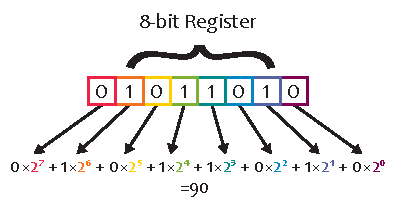
\includegraphics[width=0.75\linewidth]{Binary}
  \caption[Binary Coding]
  {We can encode information in a register in many ways. One encoding for positive numbers is to use a base-2
  positional system, like above, where the binary register \texttt{01011010} is mapped to the number 90.}
  \label{fig:binary}
\end{figure}

\subsubsection{The Qubit}
A \textbf{qubit} is similar to a bit in that it has two states, $\ket{0}$ and $\ket{1}$, except unlike a bit, it is specified
by a 2-dimensional vector, and evolves according to the rules of quantum mechanics. Due to the uniquely quantum
mechanical property of \emph{superposition}, we can no longer write the state of a single qubit (which we will
denote $\psi$) as either $\ket{0}$ or $\ket{1}$. Instead, we must write down the vector sum of the two states,
which we define as follows:
\begin{align}
  \label{eqn:basisstates}
  \ket{0} = \svec{1\\0} && \ket{1} = \svec{0\\1}
\end{align}
\begin{equation}
  \ket{\psi} = \alpha \ket{0} + \beta \ket{1} = \svec{\alpha\\\beta}
\end{equation}
where $\alpha$ and $\beta$ are complex numbers. If we were to take a measurement of this quantum state,
rather than getting back the value of this vector sum, we would measure the $\ket{0}$ state with probability
$|\alpha|^2$ and the $\ket{1}$ state with probability $|\beta|^2$. Since probabilities must sum to one, we also
get a normalization condition: $|\alpha|^2 + |\beta|^2 = 1$. The quantities $\alpha$ and $\beta$ are called
probability amplitudes, and they can take both positive and negative complex values
\footnote{Interestingly, the "complex" part of that state is unnessecary to get the extra computing power
  of a quantum computer\cite{doi:10.1142/S0219749913500019}. There's a good reason that quantum mechanics
  uses complex probability amplitudes\cite{2004quant.ph..1062A}, but if they were real, it turns out
  we can still do computations in \textsc{BQP} efficiently.}
as long as the sum of their squared magnitudes to one. This gives us the first hint as to why quantum computing
might give us more power than a classical computer: their states can interact in a manner which mirrors
interference!

\begin{figure}
  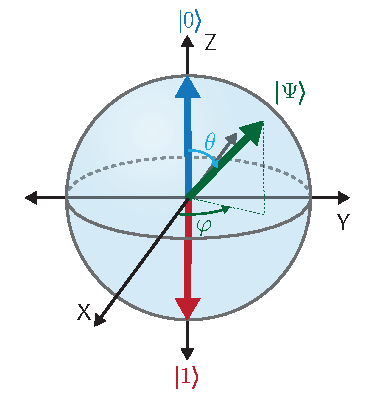
\includegraphics[width=0.5\linewidth]{BlochSphere}
  \caption[The Bloch Sphere representation of a qubit]
  {The state of a qubit can be represented as vector on the surface of a unit sphere. In this description,
  the state is described by two angles: $\theta$ and $\psi$.}
  \label{fig:bloch}
\end{figure}

Too see how this is true, it's helpful to rewrite the above state in spherical coordinates. First, let's
write $\alpha = r_0e^{-i\varphi_1}$ and $\beta = r_1e^{-i\varphi_2}$. The normalization condition is now
$r_0^2 + r_1^2 = 1$, from which we can make the replacement $r_0 = \cos(\theta/2)$ and $r_1 = \sin(\theta/2)$.
We can also factor out the phase $\varphi_1$ to give:
\begin{equation}
\ket{\psi} = e^{-i\varphi_1}\left(
    \cos\left(\frac{\theta}{2}\right)\ket{0} + e^{-i(\varphi_2 - \varphi_1)}\sin\left(\frac{\theta}{2}\right)\ket{1}
  \right)
\end{equation}
The term $e^{-i\varphi_1}$ is called a global phase factor, and is equivalent to a multiplication by a unit vector,
which it's easy to see makes no difference to the probabilities of any measurement (a fact that will continue to be
true even when we add more qubits). Another way of saying this is that the important information is encoded in
the relative phase between the two states. So, let's make the replacement $\phi = \varphi_2 - \varphi_1$ and ignore
the global phase factor, which gives us the state:
\begin{equation}
  \ket{\psi} = \cos\left(\frac{\theta}{2}\right)\ket{0} + e^{-i\phi}\sin\left(\frac{\theta}{2}\right)\ket{1}
\end{equation}
This representation is shown visially in figure~\ref{fig:bloch} and is called the Bloch sphere representation
of a qubit.

Given this description, we can now start to think about what operations on a single qubit might look like.
While on a single bit, the only non-trivial operation we can perform is a flip ($0 \rightarrow 1$ and $1 \rightarrow 0$),
on a qubit we have a whole host of operations that we can perform. The only limits we put on ourselves is that these operations
must leave us on the surface of the Bloch sphere. In other words, after applying an operation, we must still
have a normalized state. From the Bloch representation, you may have already guessed that this means we
can only perform rotations.

Switching back to the 2D vector representation of a qubit, then it's also clear that these operations
must correspond to $2\times2$ matrices. The act of performing an operation corresponds to multiplying
the qubit state by one of these matrices. To ensure that the length of the qubit vector $\ket{\psi}$
remains one at all times, the matrices we can use on our qubit must be unitary. That is, given the matrix $\boldsymbol{M}$,
its complex conjugate transpose $\boldsymbol{M}^\dagger = (\boldsymbol{M^{*}})^\mathrm{T}$ times itself is equal to
the identity matrix: $\boldsymbol{M}^\dagger\boldsymbol{M} = \boldsymbol{I}$.

Let's define three unit rotation matrices as $\pi$ rotations around the $X, Y, Z$ axes. These have the symbols
$\sigma_X, \sigma_Y, \sigma_Z$ respectively, and are called the Pauli matrices.
They have the values:
\begin{align}
  \sigma_X = \svec{0&1\\1&0} && \sigma_Y = \svec{0&-i\\i&0} && \sigma_Z = \svec{1&0\\0&-1}
\end{align}

We can build up arbitrary rotations from these unit vectors by taking various powers of these vectors
and multiplying them together. For example to apply a $\pi/2$ rotation around the y-axis applied to the state $\ket{\psi}$
we would perform $\sqrt{\sigma_Y}\ket{\psi}$. \footnote{For those familiar with the rotation operators,
this is more commonly written with a phase factor to make the solution purely real: $R_Y(\tfrac{\theta}{2})
= \exp(-i\pi/4)\sqrt{\sigma_Y}$}
A $2\pi$ rotation around the x-axis would be $\sigma_X\sigma_X\ket{\psi}$. It is possible to generalize this
to arbitrary rotations, giving us the rotation operators\cite{Nielsen:rot}:
\begin{align}
  R_X(\theta) = e^{-i \theta X/2} = \cos\left(\frac{\theta}{2}\right)\boldsymbol{I} - i \sin\left(\frac{\theta}{2}\right)\sigma_X \\
  R_Y(\theta) = e^{-i \theta Y/2} = \cos\left(\frac{\theta}{2}\right)\boldsymbol{I} - i \sin\left(\frac{\theta}{2}\right)\sigma_Y \\
  R_Z(\theta) = e^{-i \theta Z/2} = \cos\left(\frac{\theta}{2}\right)\boldsymbol{I} - i \sin\left(\frac{\theta}{2}\right)\sigma_Z
\end{align}
These three rotations (and often a global phase factor to simplify our result) are sufficient to express
any single qubit operation. For completeness, we can also define some other gates that often come up in
the context of quantum computation:
\begin{alignat}{4}
    H &=& \frac{1}{\sqrt{2}}\svec{1&1\\1&-1} &=& e^{\tfrac{i\pi}{2}} R_Y\left(\frac{\pi}{2}\right) R_Z(\pi) &=& \frac{\sigma_X+\sigma_Z}{\sqrt{2}} \\
    T &=& \svec{1&0\\0&e^{\tfrac{i\pi}{4}}}  &=& e^{\tfrac{i\pi}{8}} R_Z\left(\frac{\pi}{4}\right)          &=& \sqrt[4]{\sigma_Z} \\
    S &=& \svec{1&0\\0&i}                    &=& e^{\frac{i \pi}{4}} R_Z\left(\frac{\pi}{2}\right)          &=& \sqrt{\sigma_Z}
\end{alignat}
These are the Hadamard gate, the T gate (or $\pi/8$ gate)\footnote{The $T$-gate is often
referred to as the $\pi/8$ gate, even though it represents a $\pi/4$ rotation, a name that is derived from
the phase factor for historical reasons.} and the phase gate respectively.
As is typical, phase factors are usually dropped (something I did not do in the above), hence it is
common to see variations of these equations in the literature.

As a final example, let's take a detailed look at where interfering probabilities leads to a thoroughly
non-classical result. To start with, let's define two additional states:
\begin{align}
  \ket{+} = \frac{\ket{0} + \ket{1}}{\sqrt{2}} && \ket{-} = \frac{\ket{0} - \ket{1}}{\sqrt{2}}
\end{align}
We can get these states by starting from $\ket{0}$ and rotating $\pi/2$ or $-\pi/2$ around the Y-axis. You can
reasonably easily confirm that they are properly normalized, and that if we were to measure each state, the
probability of measuring a $\ket{0}$ or a $\ket{1}$ are equal for both states: $\mathrm{P}\left(\ket{0}\right) =
\mathrm{P}\left(\ket{1}\right) = 0.5$. So a direct measurement would be unable to distinguish these two states.
However, if we were to apply the Hadamard gate to each of those two states, we surprisingly end up with two
different outputs:
\begin{align}
  H\ket{+} = \ket{0} && H\ket{-} = \ket{1}
\end{align}
In this case, the complex probability amplitudes can interfere with each other causing the two states to
become distinguishable, something that a classical bit could not replicate. What you see is what you get.

\subsubsection{Multi-Qubit States (Qubit Registers)}
The next additional computational resource that quantum physics gives us is \emph{entanglement}. This
resource rears it's head when we try to combine multiple qubits into a register. Formally,
we can define entanglement as a correlation between the states of qubits after they have interacted
with each other. Due to this correlation, the state of a qubit that has been entangled with its partner
can no longer be described independently, the states of the two qubits become linked. Perhaps the easiest
way to grok the consequences of this is to give an example of how this correlation might play out.

Let's start with two qubits, one of which starts in the $\ket{+}$ state, the other which starts in
the $\ket{0}$ state. If we were to apply a gate that flips the state of the second qubit if the state of
the first qubit is $\ket{1}$, then we might expect to end up with something like $\ket{+}$ in the second
qubit. If we measure the first qubit and get the result $\ket{0}$, the state of the second qubit must also
be zero, so the state of the second qubit can't have been described by $\ket{+}$. The state of the two
qubits is correlated and depend on each other. The operation we described above is called the
controlled-NOT ($CNOT$) gate, and creates a state that looks like:
\begin{equation}
  \ket{\psi} = \frac{\ket{00} + \ket{11}}{\sqrt{2}}
\end{equation}
To describe a generalized two-qubit state, we must give coefficients to each possible state the qubits
can take:
\begin{equation}
  \ket{\psi} = \alpha\ket{00} + \beta\ket{01} + \gamma\ket{10} + \delta\ket{11} =
    \svec{\alpha\\\beta\\\gamma\\\delta}
\end{equation}
So to combine two qubits together, we cannot just list the states of the two qubits one after another,
they are described by the tensor product of the two individual states: $\ket{\psi} = \ket{\psi_1}\otimes\ket{\psi_2}$.
For a three-qubit register, the total number of states we must give coefficients to is 8. For a $N$ qubit
register, the total number of coefficients is $2^N$. Note the distinction between a classical register
and a quantum register, to describe a classical register, we can list the states of the individual
bits one after another, whereas the quantum register requires $2^N$ complex numbers to express fully.

Much like a single qubit, we require new matrices that can operate on quantum registers. As one
might expect, the size of these matrices is exponential in the number of qubits that we must operate on.
For example, on a two-qubit register, we require a $4 \times 4$ matrix to describe operations. The
$CNOT$-gate that we used above is defined as:
\begin{equation}
  CNOT = \svec{1&0&0&0\\0&1&0&0\\0&0&0&1\\0&0&1&0}
\end{equation}
Unfortunately, the potential presence of entanglement means applying single or two-qubit gates to a subset
of qubits in the register is no longer a matter of applying a $2 \times 2$ or $4 \times 4$ matrix, we must
construct a $2^N \times 2^N$ matrix and apply that to the full quantum register. This construction is achieved
by taking the Kronecker product of identity matrices and the matrix we want to apply. For example, to apply
a $\sigma_X$ gate to the 2nd qubit in a three-qubit register, we construct the operator as follows:
\begin{equation}
  \sigma_{X,2} = \boldsymbol{I} \otimes \sigma_X \otimes \boldsymbol{I}
\end{equation}

The consequences of the twin effects of superposition and entanglement lead to the extra computational
power of a quantum computer, while also hinting at the difficulty of writing quantum algorithms. As we
can prepare arbitrary superposition states, we can encode an exponentially large
state into a quantum register, for example representing every number between 0 and $2^N-1$ in a $N$ qubit
register, and operate on all of these states in parallel. However, once we measure the register, we end up
with only one of the possible states in the register (i.e. the state collapses), and the quantum information
that was prepared in the state is lost. Quantum algorithms must, therefore, have three properties to be useful:
\begin{enumerate}
  \item An efficient way of preparing a state. If we want to perform computations on a quantum register
    storing $2^N$ values, we lose any exponential speedup if we need to load each of these values one-by-one.
    For example, Shor's algorithm relies on being able to prepare an equal superposition of all states
    in the register with $N$ single qubit gates\cite{PhysRevA.54.1034}.
  \item Creation of a large entangled state. Without entanglement, a quantum algorithm can be efficiently
    simulated on a classical computer. The exact role that entanglement plays in computation is not yet known;
    however, without using it, we know that quantum computers lose their advantage\cite{doi:10.1098/rspa.2002.1097}.
  \item A way of whittling down the quantum state to make the "answer" the likely outcome of any readout.
    Since coefficients in a quantum register represent probability amplitudes that measurement will yield
    a given outcome, we can get at most $N$ bits of data per measurement\cite{651037}, as our register
    immediately collapses into one state upon measurement. To get another value out of the register,
    we must repeat the whole computation, including loading the state.
\end{enumerate}

\subsubsection{Noise}

\begin{figure}
  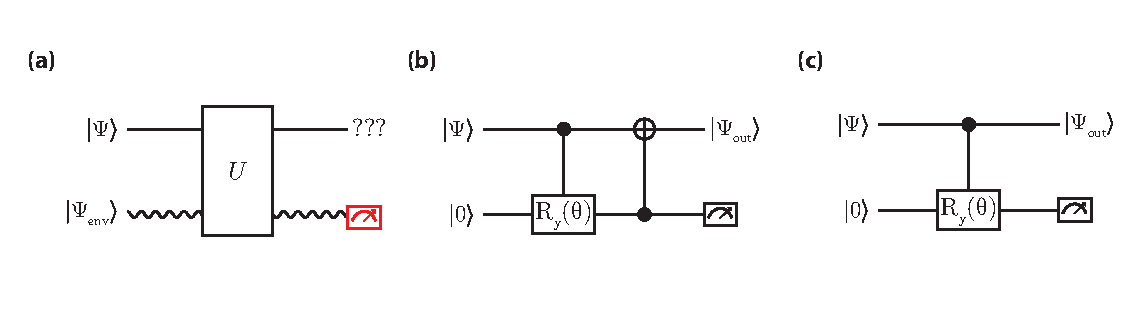
\includegraphics[width=\linewidth]{Noise}
  \caption[Noise affecting pure states]
  {(a)We can think of noise as uncontrolled interactions with an environment. However since we can't measure
  information that is transferred into the environment, we end up with an incomplete representation of our qubit.
  In order to represent this state, with some of it's information lost, we must describe the state with a density
  matrix representation. (b) A simple model for relaxation, where we represent the probability of a decay $\gamma$
  in the rotation angle $\sin^2(\theta/2) = \gamma$. Each time this gate is applied, we end up more likely to be in
  the $\ket{1}$ state. (c) A simple model for dephasing, where the phase $\theta$ is a random variable. This type
  of quantum noise has no classical analog, but causes a loss of information about the relative phase between $\ket{0}$
  and $\ket{1}$.}
  \label{fig:noise}
\end{figure}

Up to this point we have assumed that there are no noise sources or sources of information loss in our
qubit implementations. Unfortunately, reality is not so kind, and as has been discussed before, it is the
fragility of a quantum state that remains the main challenge of implementing a large scale quantum computing.
Another way of stating the same thing is to say uncontrolled coupling to the environment, either through
energy loss or uncontrolled rotations, leads to loss of information from our quantum computing, shown schematically
in figure~\ref{fig:noise}. As we are unable to make a good projective measurement of the environment, the output
state after the unitary interaction $U$ with the environment cannot be well described in the vector notation we
described above, and some information about the state is irreversibly lost. As such, the challenge of including
these sources of noise into our model of quantum computing is to figure out how to model an uncontrolled environment.
\footnote{Or, we could replace the environment with something we CAN control and measure, an approach attempted
in~\cite{2018arXiv180300545M}.}
To model this sort of interaction, we could switch to a density matrix representation of our state, which allows us
to describe a subsystem of a composite quantum system, i.e. to ignore the portion of the state lost to the environment.
Indeed this is the most complete way to describe noise processes and information loss of our state, however rather
than introduce a more powerful, but otherwise equivalent, description of quantum mechanics, we can instead model
noise processes as interactions with a controlled environment, such as another qubit, as in figs.~\ref{fig:noise} (b) and (c).
We can categorize interactions of our qubits into two general classes: relaxation (sometimes called amplitude
damping), and dephasing (sometimes called phase damping).

The first class of error, \textbf{relaxation}, causes our population to decay towards the ground state $\ket{0}$ each time it is
applied with probability $\gamma$. We can think about this sort of process as a loss of energy from the qubit system, and
in a way is analogous to classical relaxation for example of an pendulum which gradually loses energy to the environment
or an atom in an excited state that decays. An equivalent circuit for such a process into a controlled environment (a second qubit) is
shown in Fig~\ref{fig:noise} (b), where the portion of the state in $\ket{1}$ undergoes a gradual rotation $R_{y}(\theta)$
towards the $\ket{0}$ state, where the phase $\theta$ is chosen to represent the probability of a relaxation event:
$\sin^2(\theta/2) = \gamma$. We represent the permanent loss of the information as a projetive measurement made on the
second qubit. This error is commonly quoted in literature as a $T_1$ time, where $T_1$ is a time constant
that gives us the rate at which a state will decay towards the ground state:
\begin{equation}
  P(\ket{1} \rightarrow \ket{0}, t) = 1 - e^{-t/T_1}
\end{equation}

The second form of error, \textbf{dephasing}, is one that does NOT have a classical analog, and represents randomization of the phase between
states in the qubit or qubit register. Understanding the effect of this sort of noise is harder than for relaxation since there is no
calassical analog, however if we permit ourselves a Bloch sphere representation of a qubit, we can visualize it
as a randomization of the $\varphi$ angle. An equivalent circuit, again using a second qubit to simulate the
environment is shown in fig.~\ref{fig:noise} (c). We represent an irretrievable loss of information to the
environment as a projective measurement on the second qubit. This error rate is commonly quoted as the $T_2$ time,
the rate that phase information is lost to the environment. In the case of a single qubit, or completely uncorrelated
(markovian) noise, this would be the end of the story, however in most systems, we also define a $T_2^*$, an ensemble
dephasing time. In the case of single qubits that evolve under quasi-static noise
\footnote{Quasi-static noise is noise that is approximately constant over the timescale of qubit operations. More formally,
we can define it as non-markovian noise, that is there is some correlation in the noise that we can learn and correct
by appriate application of dynamical decoupling.} or multi-qubit systems that operate
under an inhomogeneous background, we can use correlations in the noise or the static nature of the inhomogeneous background
to "rephase" our qubits~\cite{PhysRev.80.580,dynamic-decoupling-biercuk}. We can think of this effect as coming from the
fact that the phase evolves at a constant rate over the timescale of operations, such that by applying an $X$ gate to our
qubit/qubits, we can unroll whatever phase was accumulated.  In this case, the $T_2$ time becomes the relaxation rate after
application of rephasing gates, while $T_2^*$ is the ensemble dephasing time, assuming measurement over a longer timescale
than the correlation time and without correcting for inhomogeneities.

% Possible TODO: Circuit notation?

\section{Making Qubits in Semiconductors}
\label{sec:qcinsm}
Having described the basic ideas of quantum computing, our next challenge is to find a physical system that
is able to implement the operations that we discussed above. This problem can be distilled to that
of finding a quantum two-level system that follows a set of criteria that were first laid out by David
DiVincenzo, a criteria that is widely considered to be the standard checklist for any qubit\cite{divincenzo_crit}. They are:
\begin{enumerate}
  \item A scalable physical system with well characterized qubits
  \item The ability to initialize a fiducial qubit state, such that the state of the system is known prior
    to any quantum operations.
  \item Decoherence time in the qubit subspace that greatly exceeds the gate operation time.
  \item A universal set of quantum gates.
  \item The ability to perform measurements on individual qubits.
\end{enumerate}
Although these criteria set out some requirements for useful qubits, they are certainly not so prescriptive
that there is a dearth of systems that could fulfil them. It is in this context that ion-traps, photonic,
NMR based qubits, superconducting and semiconductor based qubits are being invevstigated, each with advantages
and disadvantages for each criterion. Apart from a brief discussion of the scalability prospects of each of these systems
in section~\ref{sec:arch}, I will focus on semiconductor based qubits for the remainder of this thesis. This type
of qubit has the potential to utilize the extroadinary processing capabilities of modern semiconductor manufacturing
although as we shall see, even within this subset of possible qubit systems, there are still many different
choices of two-level subspace. As a result, I will not attempt to comprehensively cover all the variations
of qubit that exist, rather I will focus specifically on two general designs, quantum dots and majorana zero modes,
which in many ways share similar control and readout. This also means that the discussion of physics in this section will
largely be confined to III-V materials, although I will point out that as my thesis is aimed at the general
problem of architecting a quantum computer, many of the results presented may find use outside the subset of physics
I present here. Before we begin a detailed discussion of qubits in semiconductors, let's first take a look
at the physics that underlie most of these implementations; the 2-dimensional electron gas (2DEG).

\subsection{The 2-Dimensional Electron Gas}
The 2-dimensional electron gas (2DEG) is the foundation for many of the experiments and qubit-realizations
that follow, and is a way of confining electrons in a semiconductor to a single plane. In order to fully
appreciate what this means, we first have to discuss what it means to confine an electron in one of the three dimensions.
How big does this confining potential have to be? To answer this question, we must first look at the solutions
to Schr\"odinger's equation in a semiconductor. This will give us the form of the electron wavefunction, and
an idea of its "size". The following introduction is based on material taken from~\cite{delftbook,ihnbook,Ashcroft}.

\begin{figure}
  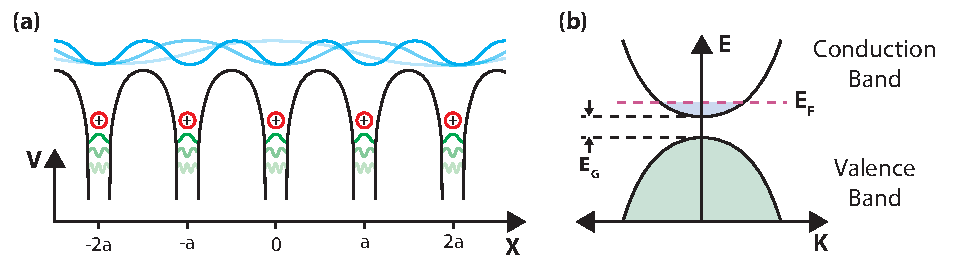
\includegraphics[width=0.9\linewidth]{BlochWaves}
  \caption[Bloch Waves on a regular lattice]
  {(a) Given a periodic lattice that creates a set of potential wells, the valid solutions for unbound
   electrons (conduction band) are plane waves with a period proportional to the lattice spacing ($a$),
   while bound electrons (valence band) are proportional to the binding material. (b) Assuming there are no
   electron-electron interactions ($E_\textrm{F}$).}
  \label{fig:blochwaves}
\end{figure}

In a crystalline material, such as a metal or a semiconductor lattice, we can think
about electrons as travelling along a periodic potential, caused by the periodic spacing of nuclei in the lattice, as
is shown in figure~\ref{fig:blochwaves}~(a) for a 1D lattice. There will be two sets of solutions, the first will be for electrons
that are tightly bound around nuclei, which will form the valence band, and free electron solutions which
will form the conduction band. The gap between these two solutions forms a band gap of size $(E_G)$, a range
of energies for which there are no available states. As we are looking at the 2DEG, let's focus on free electron solutions for now.
These will take the form of Bloch waves, expressed as a function of lattice position $r$ and wave vector $k$:
\begin{equation}
  \psi_{\vec{k}}(\vec{r}) = e^{i\vec{k} \cdot \vec{r}}u_k(\vec{r})
\end{equation}
where $u_k$ is a periodic function with the same periodicity as the crystal lattice and $\exp\left(i\vec{k} \cdot \vec{r}\right)$ are
plane wave solutions. What this equation effectively says is that if we are able to solve around boundary conditions for
a single unit cell, we can extract a band structure for the entire lattice.

Electrons in this system begin to fill the available states from the lowest energy up, obeying the Pauli exclusion principle which limits
each available state to two electrons with opposite spins. For conduction band electrons in regular crystals we can make
two additional assumptions that aid in the interpretation of the solutions to the bloch equation. First, let's assume that
there are no electron-electron interactions. Although this assumption may at first be unintuitive, it appears
to be sufficient to describe much of the physics that follows. Second, we assume that the potential due to the
lattice is screened by valence band electrons, and can be treated as a peturbation to a free electron. Solving
this model leads to bands which are similar to free electron plane waves up to the edge of the Brouillin zone, i.e.
up to the top of the band. In the conduction band of a semiconductor, we deal with largely empty bands, as such
the dispersion relation, i.e. theenergy of electrons as a function of wave vector, can be approximated as that of free electrons:
\begin{equation}
  E\left(\vec{k}\right) = \frac{\hbar^2 |\vec{k}|^2}{2m^*}
\end{equation}
where $\vec{k}$ is the electron wave vector and $m^*$ is the effective electron mass. From this, we can also give the
formal definition for the Fermi energy. The \textbf{Fermi energy} ($E_F$) is the highest filled electronic state
at zero temperature. This situation is represented schematically in figure~\ref{fig:blochwaves}~(b) for a single dimension.
In 3D, the Fermi energy forms a sphere in momentum space dilineating the region where electron states are filled, the surface
of which we call the Fermi surface. From this, we can define the Fermi wavelength $\lambda_F$ of an electron at the Fermi
surface, effectively the size of an electron in our semiconductor. Using $k = 2\pi/\lambda$ we find:
\begin{equation}
  \lambda_F = \frac{h}{\sqrt{2m^*E_F}}
\end{equation}

\begin{table}
  \centering
  \begin{tabular}{|l|l|l|}
   \hline
   Crystal & Lattice Constant (\si{\angstrom}) & Electron Effective Mass$(m^*/m_e)$ \\
   \hline
   Si & 5.43 & - \\
   Ge & 5.658 & - \\
   GaAs & 5.65 & 0.066 \\
   InAs & 6.06 & 0.026 \\
   InSb & 6.48 & 0.015 \\
   \hline
  \end{tabular}
  \caption[Properties of some common Semiconductors]
  {Lattice constants and effective electron masses for some common semiconductors. For Si and Ge semiconductors, which are
  indirect band gap semiconductors, the effective mass for electrons is not trivial and will vary based
  on direction and valley state, hence values are not given above. Values are taken from~\cite{Kittel2004,InSbParam}.}
  \label{tab:semiprop}
\end{table}

If we wish to confine electrons in a given dimension, this gives us the relevant length-scale over which it must became
done. For metals, the large number of free electrons means the Fermi energy is large, and as such we end up with a
Fermi wavelength on the order of a few Ångström (where $\SI{1}{\angstrom} = \SI{1e-10}{\meter}$). In semiconductors, as
the number of free electrons, and hence the Fermi energy, is set by the doping and is generally small, the Fermi
wavelength can be on the order of a few 10s of nanometers. Paramters for some common semiconductors are given
in table~\ref{tab:semiprop}. Given these values, if we can make a potential well with a width $W$ that's on
the order of the Fermi wavelength, we are able to confine electrons to a few subbands. The next question is: how
do we create a narrow quantum well?

\begin{figure}
  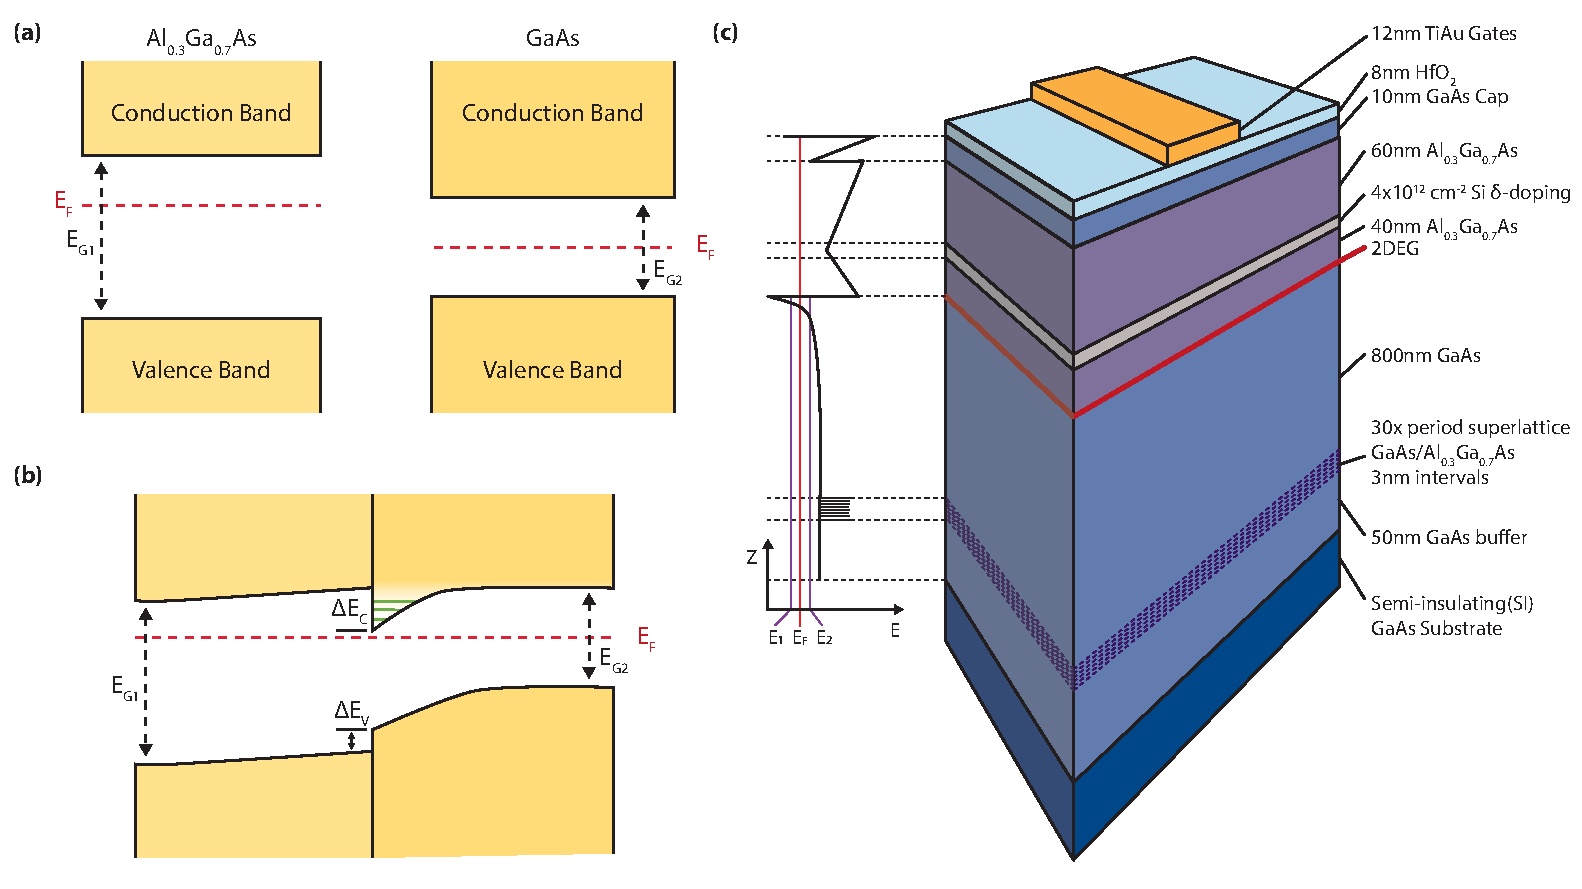
\includegraphics[width=1\linewidth]{GaAs}
  \caption[Band bending in a straddling type heterojunction, and the GaAs/AlGaAs heterostructure]
  {\label{fig:heterostructure}(a) Shows a straddling type heterojunction between \ce{Al_{0.3}Ga_{0.7}As} and GaAs with two
  differing bandgaps $E_{G1}$ and $E_{G2}$, where the smaller gap ($E_{G2}$) is fully enclosed in the larger gap $E_{G1}$.
  (b) When the two semiconductors are equalized, their bands bend near the heterojunction to ensure a continuous Fermi
  energy. Far from the junction, the unmodified band structure is restored. (c) The layer stack of a GaAs/(Al,Ga)As heterostructure,
  with TiAu surface gates that can locally modify the density of the 2DEG.}
\end{figure}

The answer is to create a heterojunction; an interface between two dissimilar semiconductors with different band-gaps. The
simplest type of heterojunction we can form is a straddling (type I) junction, where one semiconductor has a smaller band-gap
that is contained within the band gap of the other, a situation that is represented schematically in fig.~\ref{fig:heterostructure}.
In the case that the Fermi levels of the two semiconductors is unequal, electrons tunnel between the two junctions in order to align
their levels, leading to band bending at the interface. Careful choice of semiconductors can cause a well to appear at the interface,
where the width of the well can be designed to be on the order of the Fermi wavelength in the semiconductor. GaAs and (Al,Ga)As are
an ideal choice for this type of heterojunction as  they are almost perfectly lattice matched (their lattice constants differ by 0.14\%),
while also forming a straddling-gap heterojunction with a gap in GaAs $E_{G1} = \SI{1.424}{\electronvolt}$ and a gap in
\ce{Al_{1-x}Ga_{x}As} that can be continuously varied, taking the value $E_{G2} = 1.424 + 1.225x$ \si{\electronvolt}, by
changing the ratio of Al and Ga in the semiconductor. Furthermore, up to $x = 0.44$, the ratio of the step in the conductance
band ($\Delta E_C$) to the step in valence band ($\Delta E_V$) is a constant: $\Delta E_C/\Delta E_V = 1.5$~\cite{adachi1993properties}
[see steps in figure~\ref{fig:heterostructure}~(b)], allowing the depth of the well to be easily varied.
Finally, by doping the semiconductor with Si, we are able to move the Fermi energy up to populate a single subband, leading to a
2-dimensional plane of electrons, where there is only a single wavevector in the Z direction ($k_z$) that electrons can take. As long
as the electron temperature is far below the energy, only this subband will be populated.

The structure of a typical GaAs/\ce{Al_{0.3}Ga_{0.7}As} heterostructure is shown in Fig.~\ref{fig:heterostructure}~(c). Such structures
are normally grown by molecular-beam epitaxy (MBE) which allows atomically smooth layers to be grown a single monolayer
at a time. Heterostructures are grown on a semi-insulating GaAs substrate, ober which a large buffer is grown.
Repeated thin layers of GaAs/\ce{Al_{0.3}Ga_{0.7}As} are grown in order to reduce the dislocation density
and create a continuous, smooth single crystal at the heterojunction. The 2DEG itself is represented by the red line
on the schematic, where it is followed by a region of Si $\delta$-doping, used to pin the Fermi level in the substrate, and
a \SI{10}{\nano\meter} GaAs cap to protect against oxidation. During processing, a protective oxide barrier (either \ce{HfO2}
or \ce{Al2O3}) is grown, followed by surface gates which allow the density of states to be locally modified, or even depleted,
in order to form structures in the 2DEG. The oxide layer, apart from serving as a passivation barrier, is also necessary to
prevent tunneling of electrons from the surface gates into the donor layer, where movement of electrons is known to be a significant
source of charge noise~\cite{PhysRevB.72.115331,PhysRevApplied.9.034008}.

Having strongly confined electrons into 2-dimensions, we can now redefine several of the parameters that we had above. First, our
dispersion relation becomes that of free electrons in two-dimensions:
\begin{align}
  E(\vec{k}) = \frac{\hbar^2 |\vec{k}|^2}{2m^*} && |\vec{k}|^2 = k_x^2 + k_y^2
  \label{eq:k2d}
\end{align}

We can also define the density of states (DOS) in 2-dimensions as the number of states $n(E)$ per unit energy $(E)$:
\begin{equation}
  \rho_{2D} = \frac{d n(E)}{d E}
\end{equation}

For free electrons in 2D, the states fill an area in momentum-space up to k-vector $k$:
\begin{equation}
  A = \pi k^2 = \frac{2 \pi m^* E}{\hbar^2}
\end{equation}
where we've substituted equation~\ref{eq:k2d} for $k$. The spacing of states in a crystal of size $L \times L$ is given
by $\pi^2/4 L^2$, so for a unit area, the area of a single state is $A_{\textrm{single}} = \pi^2/4$. Putting this together,
the number of states up to energy $E$ is therefore:
\begin{equation}
  n(E) = g_s g_v \frac{A}{A_{\textrm{single}}} = g_s g_v \frac{m^* E}{2 \pi \hbar^2}
\end{equation}
and giving a density of states:
\begin{equation}
  \rho_{2D} = g_s g_v \frac{m}{2 \pi \hbar^2}
\end{equation}
where $g_s$ is the spin degeneracy (almost always 2), and $g_v$ is the valley degeneracy (1 for III-V semiconductors, 3 for Si).
Importantly we note that the density of states is independant of energy, a situation which is unique to 2-dimensions. This allows
us to redefine the Fermi energy, wave-vector and wavelength in terms of the total electron density ($n_s$) rather simply:
\begin{align}
  E_F = \frac{n_s}{\rho_{2D}} = \frac{2 \pi \hbar^2 n_s}{m^* g_s g_v} &&
  k_F = \sqrt{\frac{4 \pi n_s}{g_v g_s}} &&
  \lambda_F = \sqrt{\frac{\pi g_s g_v}{n_s}}
\end{align}

Up till now, we've been focused on systems at zero temperature and without the effects of scattering. We can modify our above
descriptions of various effects while accounting for temperature and scattering without a huge amount of extra effort.
First, the main effect of temperature will be to create s distribution of filled states around the Fermi energy, rather
than a sharp cut-off as we had previously assumed. This distribution takes the form:
\begin{equation}
  f(E - E_F) = \left[1 + \exp\left(\frac{E - E_F}{k_B T}\right)\right]^{-1}
\end{equation}
This places an additional constraint on 2DEG formation, namely that the thermal energy $k_B T$ should be much less than the
2D subband spacing, a requirement that is easily met for most heterostructures below a few Kelvin. Second, we account for the
effect of scattering. This is commonly captured in a length that an electron can travel before scattering. Depending on the scattering
mechanism this can either be inelastic, normally due to scattering of phonons (thermal scattering), or elastic, normally due to
scattering off lattice defects or impurities. We therefore define two length scales, $l_\psi$ being the inelastic scattering length,
which gives us the length scale over which total kinetic energy and momentum are conserved, and $l_e$ being the elastic scattering
length, which gives the length of time an electron will travel before any collision. This also sets a momentum relaxation time, the
amount of time between electron collusions given by $\tau = l_e/v_F$.

In general, we are more interested in the effect of scattering on conductivity, an easily measured bulk property of
the semiconductor. We can reframe the scattering time into a conductivity by considering the motion of an electron
through a lattice. Let's define a quantity called the drift velocity $v_d$ as the average speed an electron moves through
the lattice under an accelerating field $E$. Then, by Newton's second law:
\begin{equation}
  eE = \frac{m^* v_d}{\tau}
\end{equation}
If we rearrange for $v_d$ we find:
\begin{align}
  && v_d = \mu E && (\textrm{where~} \mu = \frac{e \tau}{m^*})
\end{align}
where $\mu$ is a quantity called mobility, with units \si{\square\centi\meter\per\volt\per\second}.
Then to find the conductivity, we remember the definition for current
density, which will be given by the number of electrons that pass an area per second, $J = n_s e v_d$, and the definition
of conductivity, which is simply current density per electric field, $\sigma = J/E$. This gives and equation for conductivity
in terms of electron density and mobility as:
\begin{equation}
  \sigma = n_s e \mu
\end{equation}

At this point, our discussion splits into two streams.
The first deals with the formation of quantum dots, that is structures with tight confinement in all three dimensions,
and is covered in section~\ref{sec:qd}.
The second deals with characterization of 2DEGs, extracting
mobility, density, strength of the spin-orbit interaction and so forth, and is covered in section~\ref{sec:char}.
Both of these are crucially important for building a variety of qubits in semiconductors,
and many of the advances in the construction of both spin qubits and topological qubits stem from improvements in
materials science that have led to higher quality 2DEGs and the availability of exotic material systems.

\subsection{Quantum Dots}
\label{sec:qd}
Let's now consider the question of how we might use the 2DEG to form a qubit. This can occur in many different
ways, for example through the creation of superconducting Josephson junctions with a 2DEG to tune the Josephson
energy~\cite{karl-gatemon} or in Majorana zero modes\cite{PhysRevLett.119.136803}, formed using a 2DEG as a starting
point, a topic we shall explore in section~\ref{sec:majo}. By far the most well studied is to use a 2DEG to confine
electrons in a zero-dimensional quantum dot, using surface gates to define zero-dimensional "puddles" of electrons
~\cite{RevModPhys.79.1217,RevModPhys.75.1}.
These puddles of electrons, which in a semiconductor have dimensions on the order of the Fermi wavelength $\lambda_F$,
creates a discrete spectrum of available states, a situation akin to having an atom with a set of orbital modes
stuck in the middle of your 2DEG\cite{PhysRevLett.77.3613}. Before considering a quantum dot in a semiconductor, let's
start off by looking at a small metal island, which will not have well resolved orbital modes but can still contain a discrete,
well defined number of electrons.

\begin{figure}
  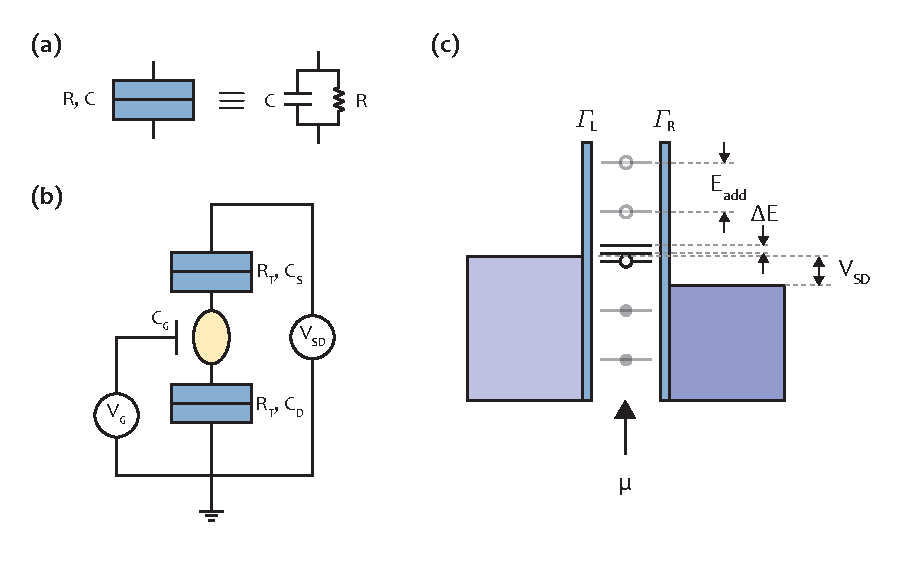
\includegraphics[width=0.8\linewidth]{Dot}
  \caption[Schematic of a Single Quantum Dot]
  {\label{fig:QD}(a) We define a tunnel junction as a combination of a resistor and a capacitor in parallel,
  since for a quantum dot the geometric capacitance of the junction is significant. (b) Equivalent circuit
  model of a quantum dot. The dot is connected to reservoirs by a source and drain tunnel junction, where
  we define the drain as ground. A voltage $V_SD$ may be applied across the quantum dot, which may cause current
  to flow. The levels of the quantum dot can be tuned by a gate voltage $V_G$ that is capacitively coupled to the
  quantum dot. (c) Schematic of a quantum dot showing a "ladder" of states, and orbital energy level. When a level
  falls within the source-drain bias window, current may flow across the dot, otherwise current is blocked, an
  effect termed Coulomb blockade.}
\end{figure}

To understand how this is possible, let's start off with the formula for the energy on a capacitor, the same one that
we initially give for a classical capacitor. This is given by: $E = Q^2/2C$. The energy to add a single extra electron
to this island is the \textbf{charging energy}:
\begin{equation}
  E_C = \frac{e^2}{2 C_{\Sigma}}
\end{equation}
where $C_\Sigma$ is the total capacitance to the dot. Let's then couple this island to two reservoirs, say a source
and a drain, both with resistance $R_t$. Realistically, these couplings add an additional capacitance term, which
we must consider in our $C_\Sigma$ term, as shown in Fig.~\ref{fig:QD} (a). We can also add a gate nearby that we can use to pull electrons on and off
the island. This situation is represented schematically in Fig.~\ref{fig:QD} (b). You might ask what differentiates
this system from a circuit I could make on my bench with three capacitors and two resistor. In other words, what are
the conditions for the number of electrons on the dot to be well defined? First off, we want the thermal energy
in the system to be much smaller than the charging energy, otherwise we won't have a well defined ground state:
\begin{equation}
  k_B T \ll E_C
\end{equation}
Next, we want to ensure that tunneling occurs at a slow rate relative to the Heisenberg uncertainty relation
$\Delta E_C \Delta t \geq h/2$, otherwise dots can hop on and off the dot faster than we could resolve them.
The tunneling time is given by $\tau = R_t C$, the time constant of the system. Combining $\tau$ and $E_C$,
we find our second restriction:
\begin{equation}
  R_t \gg h/e^2
\end{equation}
This quantity $h/e^2$ is called the von-Klitzing constant, or the quantum or resistance, and will show up
throughout this thesis in a number of contexts; as the resistance of a 1D channel, the resistance of an edge
state in the quantum Hall and spin quantum Hall effect and the tunnel rate through coupled Majorana zero modes,
and has the value $R_K = \SI{25812.807}{\ohm}$.

From here, we can define the total energy of the quantum dot with $N$ electrons. To do this we will use a
semi-classical model called the constant-interaction model. This defines the energy in terms of the background charge $N_0|e|$
\footnote{We can think of the background charge $N_0$ as the quantized equivalent of the Fermi energy. It is equivalent
to $E_F = N_0^2 E_C$, and tells us how many electrons are in the dot at zero gate voltage.},
the voltage and capacitance of the source, drain and gate, and, if we include orbital energies again, i.e. we once again work
in the limit of a small sized dot relative to the Fermi wavelength, the sum of the orbital energies $E_n(B)$, where
$E_n(B)$ is the energy of the $n$-th orbital under a magnetic field B:
\begin{equation}
  U(N) = \frac{[-|e|(N-N_0) + C_SV_S + C_DV_D + C_GV_G]^2}{C_\Sigma} + \sum_{n=1}^N E_n(B)
\end{equation}
We can also define the electrochemical potential $\mu(N)$ of the dot:
\begin{equation}
  \mu(N) \equiv U(N) - U(N-1) = \left(N - N_0 - \tfrac{1}{2}\right)E_C - \frac{E_C}{|e|}\left(C_SV_S + C_DV_D + C_GV_G\right) + E_N(B)
\end{equation}
Note that we've made the assumption that we are tunneling into the ground state of each level, it is a reasonably
simple modification to the above to calculate the chemical potential of tunnneling into an excited orbital
state. The most important difference here is a linear dependance on gate voltage, which allows us to draw
a "ladder" of states where the gap between each state is fixed at a value $E_{\textrm{add}}(N) = \mu(N+1) - \mu(N) = E_C + \Delta E_N$,
a situation depicted schematically in Fig.~\ref{fig:QD} (c). Note that the spin degeneracy of orbital states,
leads to a doublet structure in the level spacing. This equation also shows us that the electrochemical potential
of the dot can be swept linearly by varying the gate voltage.

\begin{figure}
  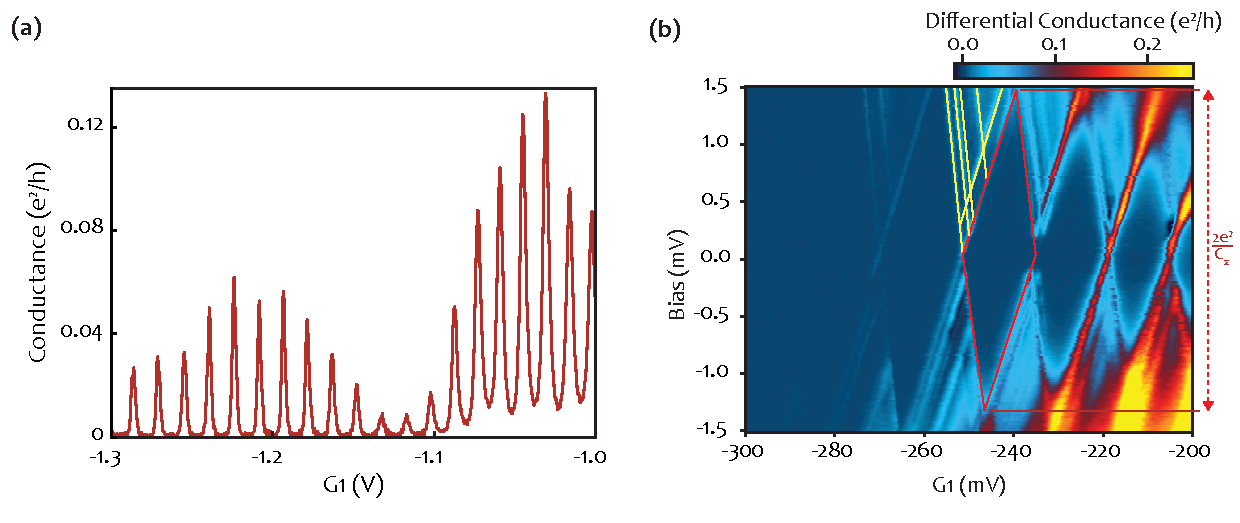
\includegraphics[width=1.0\linewidth]{CB}
  \caption[Coulomb Blockade in a Single Quantum Dot]
  {\label{fig:cbtrans}(a) Coulomb Blockade through a single quantum dot. Current can only flow at points
  where the energy levels in the dot are in alignment with the reservoirs, which occurs as the gate voltage
  is swept. (b) Sweeping bias as well as the gate, we get diamond-like features as the levels move into
  and out of the bias window. The charging energy can be extracted by looking at the width of a diamond, as
  shown in red, and increases as the size of the dot is reduced by a more negative confining potential. We can
  also see excited states within each diamond, highlighted in yellow on a single diamond. These correspond to orbital
  modes within the quantum dot.
  }
\end{figure}

The next question we might ask is how can we flow current through the dot. This can only occur via the addition of an electron
from the source ($N \rightarrow N+1$) and the removal of an electron to the drain ($N+1 \rightarrow N$), which only occurs
when the electrochemical potential $\mu(N)$ is aligned with the potential of the reservoirs for some N:
\begin{equation}
  E_F - \frac{|eV_{SD}|}{2} \leq \mu(N) \leq E_F + \frac{|eV_{SD}|}{2}
\end{equation}
This leads to a peaked conductance spectrum at low source-drain bias as a gate voltage is swept (as in Fig~\ref{fig:cbtrans} (a)), or
diamond-like regions of blocked conductance as source-drain bias is swept as a function of gate voltage (as in Fig~\ref{fig:cbtrans} (b)),
an effect termed Coulomb blockade. The spacing of coulomb diamonds allows the extraction of charging energies and addition energies, as
well as the lever arm, that is the ratio of gate capacitance to total capacitance, for each gate that is swept. The width of Coulomb
peaks also reveals information about the temperature of the electron back, as high electron temperatures smears the population in
the source and drain reservoirs. A derivation of this is not given here, however we point the curious reader to~\cite{grabert2013single},
and note that this is the method by which electron temperatures are extracted in section~\ref{sec:gb_paper}.

\subsubsection{Double Quantum Dots}
\begin{figure}
  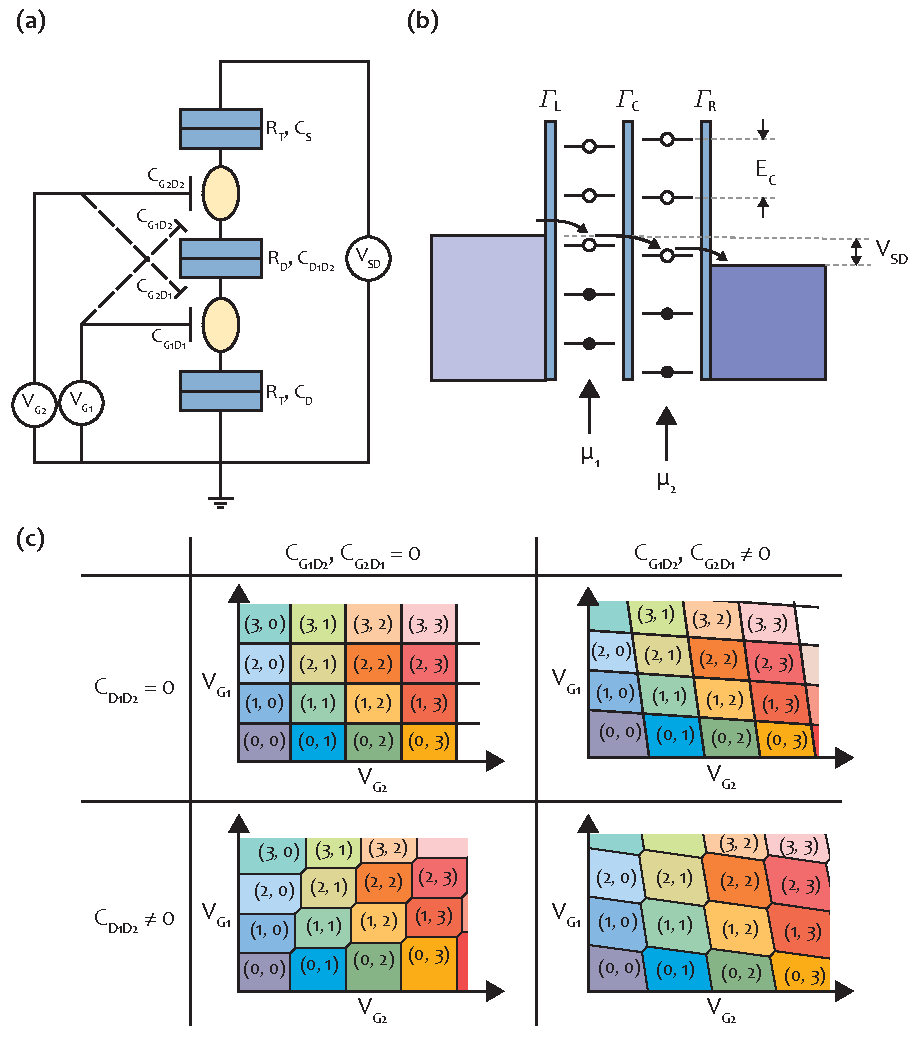
\includegraphics[width=1.0\linewidth]{DoubleDot}
  \caption[Schematic of a Double Quantum Dot]
  {\label{fig:dqd}(a) Equivalent circuit model for a double quantum dot. The circuit is very similar to that of
  two single quantum dots in series, except that we must also account for cross capacitances between adjacent gates
  (the terms $C_{G1D2}$ and $C_{G2D1}$), as well as the contribution of the tunnel junction between the left and
  right dots (the term $R_D$ and $C_{D1D2}$). (b) Energy levels in a double quantum dot system. For current to flow
  through this circuit, there must be an available level in both the left and right quantum dots. (c) Here we map
  out the effect of cross capacitance and inter-dot capacitance on the charge stability diagrams of a double quantum
  dot system as $V_{G1}$ and $V_{G2}$ are varied. As each $V_{G1}$ ($V_{G2}$) becomes more positive, more dots are
  pulled onto the left (right) quantum dot. If gate capacitance is turned on the lines take on a slope. If inter-dot
  capacitance is turned on, each stable configuration splits into a hexagonal cell. Note that these drawings do
  not include the effects of tunnelling between dots.}
\end{figure}

Having defined a single quantum dot and before we move onto a discussion of how we might use these to form qubits,
we also cover the effect of coupling two single dots together. Much like we can consider a single quantum dot an
artificial atom, so too we can consider two quantum dots that allow tunnelling of electrons between each side as
an artificial molecule. The extension of the single quantum dot picture to a double quantum dot picture occurs by
adding an additional tunnel junction between the left and right dots, and adding an additional gate to control the
electrochemical potential of the second quantum dot, as shown in the schematic in Fig.~\ref{fig:dqd} (a). In order
to fully model the effect of a double quantum dot, we must account for two additional sources of capacitance, first
a cross capacitance between the left (right) gate and the right (left) quantum dot, and second the capacitance between
the left and right dot. Intuitively we can understand the capacitance between dots as a new electron on the left dot
pushing an electron off the right dot or vice-versa, leading to a shift in the ground charge state as electrons are
pulled on and off each quantum dot. In order to characterize the effect of the two gates on a double quantum dot, we
can plot the ground state occupancy of the quantum dots as each of the gate voltages is swept. A mockup of a charge
stability diagram is shown in Fig.~\ref{fig:dqd} (c) for as both interdot capacitance and gate cross-capacitance
is turned on and off. The occupancy of the double quantum dots is labelled $(N, M)$ where $N$ represents the
occupancy of the left double quantum dot and $M$ represents the occupancy of the right double quantum dot.

As with a single quantum dot we can define the energy of the double quantum dot system using the constant
interaction model:
\begin{multline}
  U(N, M) = \frac{[-|e|(N-N_{0}) + C_SV_S + C_{G1D1}V_{G1} + C_{G2D1}V_{G2} - |e|MC_{D1D2}]^2}{C_{\Sigma,1}} \\
          + \frac{[-|e|(M-M_{0}) + C_DV_D + C_{G1D2}V_{G1} + C_{G2D2}V_{G2} - |e|NC_{D1D2}]^2}{C_{\Sigma,2}} \\
          + \sum_{n=1}^N E_{n,1}(B) + \sum_{m=1}^M E_{m,2}(B)
\end{multline}
where we have added terms $C_{G1D2}$ and $C_{G2D1}$ to represent the cross capacitance between opposite
gates and dots, and $C_{D1D2}$ is the capacitance between dots. The electrochemical potential for each dot
can also be defined in a similar way:
\begin{align}
  \mu_1(N, M) = U(N, M) - U(N-1, M) \\
  \mu_2(N, M) = U(N, M) - U(N, M-1)
\end{align}

\begin{figure}
  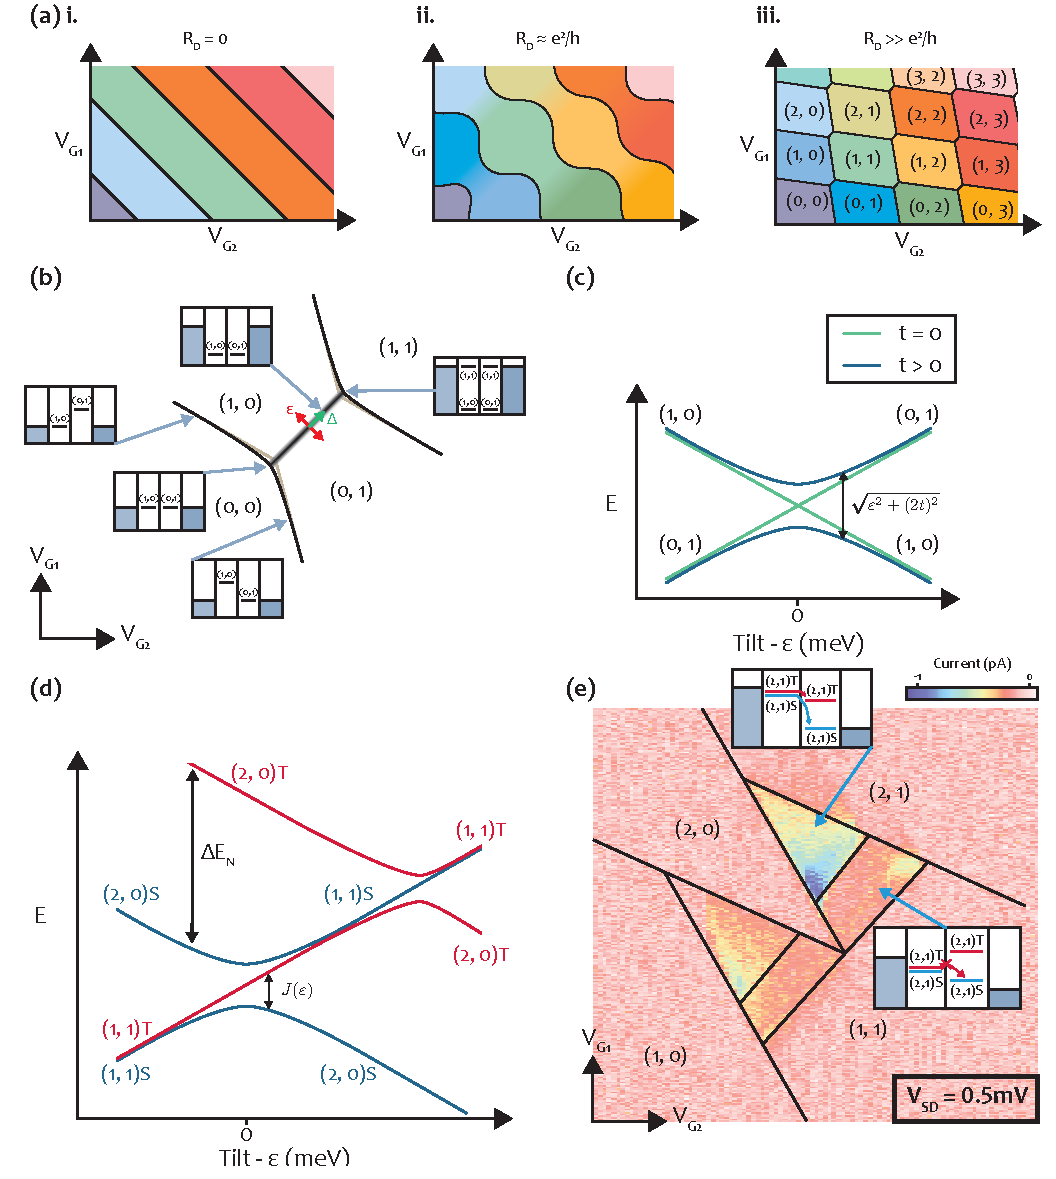
\includegraphics[width=0.9\linewidth]{ddenergy}
  \caption[Energy levels and spin in a double quantum dot]
  {\label{fig:dqdenergy}(a) Effect of varying $R_D$, the tunnel rate between the two
  dots. At low resistance the dot effectively reverts to a single quantum dot. As the resistance is increased towards
  $e^2/h$, two separated dots begin to form, although the transition between them is tunnel broadened.
  Finally, if the resistance is much larger than $e^2/h$, there are well defined transitions between left and right
  dot. (b) Zoom up of a single honeycomb cell around the $(0, 0)$, $(1, 0)$, $(0, 1)$ and $(1, 1)$ charge transitions.
  Insets show energy levels $\mu_1(N, M)$ of the left quantum dot and $\mu_2(N, M)$ of the right quantum dot where backeted
  numbers indicate the charge occupancies of both dots. We define the tilt (offset) axes perpendicular (parallel) to the
  inter-dot transition in red (green). (c) Calculated energy levels along the $(0,1) \rightarrow (1,0)$ charge transition according
  to a full quantum model. For finite tunnel coupling, an avoided crossing is formed. (d) Calculated energies of singlet and
  triplet spin configurations for a two-electron double quantum dot. Due to the Pauli exclusion principle, the $(2, 0)T$
  state is not accessible until we reach the first excited orbital state, such that the $(2, 0)T$ level is energetically
  inaccessible at zero detuning. We define the exchange energy $J(\varepsilon)$ as the energy between the $(1, 1)S$ and $(1, 1)T$
  states. (e) Current through a double quantum dot at $V_{SD} = \SI{0.5}{\milli\volt}$. Charge transitions split into finite bias triangles
  which reveal the presence of excited orbital states in the dot, as well as the effects of spin, which blocks transport through the ground
  orbital state of the dot.}
\end{figure}

The constant interaction model is limited however in describing the effect of tunelling between two dots, as the constant
interaction model assumes that the occupancy of each dot is a good quantum number, a situation which will not hold near
charge degeneracy points particularly when tunneling rates between the two dots is large. If we wish to include a finite tunnel
conductance, we must move to a Hubbard model that includes the effects quantum fluctuations, spin and orbital effects on each
dot~\cite{PhysRevB.84.115301}. In this model, and indeed in most descriptions of double quantum dot descriptions, we
describe the strength of tunnelling between the two quantum dots as a \textbf{tunnel coupling}. This model allows us to draw a schematic
of the continuous evolution from single quantum dot to double quantum dot as the strength of the inter-dot tunnel coupling
is increased. For example, Fig.~\ref{fig:dqdenergy} (a) we see evolution from the case with zero tunnel resistance i.e. a single
quantum dot in (a), to a region of intermediate tunnel resistance in ii., and finally a completely separated quantum dot in iii. Moving
towards the limit of smaller tunnel couplings (larger tunnel resistance), the bending of charge transitions will continue to be visible
in single charge transitions as in Fig~\ref{fig:dqdenergy} (b), where the constant interaction model (grey) is compared to a full quantum
treatment (black).

Examining in further detail this single honeycomb
cell in the charge stability diagrom of a dot that includes both a cross capacitance and an inter-dot capacitance, we map
out the energy levels of a quantum dot at various points according to the constant interaction model in the insets of Fig~\ref{fig:dqdenergy} (b).
In this case, looking at the $(0, 0), (0, 1), (1, 0), (1, 1)$ transition, we find two points where
three charge transitions meet, so called triple points, where energy levels within both the left and right dot are aligned
with the reservoirs. If we were to try and pass a current through such a system, it would only be at these points that a
current would flow. In between these triple points we find a new inter-dot transition, which comes from the fact that $\mu_{(1 \textrm{and} 2)}$
is now a function of gate voltage \emph{and} the occupancy of dot $(2 \textrm{and} 1)$. This leads to an additional penalty that must be
overcome to load an electron on both left and right dots, hence the point where we move from $(0, 0) \rightarrow (1, 1)$ is
pushed up in both $V_{G1}$ and $V_{G2}$. In order to further analyze this charge transition, we rotate ourselves to align with
the inter-dot transition and define two new perpendicular axes.
Tilt ($\varepsilon$) is defined as movement perpendicular to the interdot charge transition and is shown in red. It measures the relative
charge configuration of the dots ($\varepsilon = \mu_1 - \mu_2$) while keeping the overall charge of the two dots constant.
Offset ($\Delta$) is defined as movement parallel to the interdot charge transition and is shown in green.
It measures the total charge offset $\Delta = \mu_1 + \mu_2$ without modifying the relative distance between levels in the left
and right dot. In this way we can move through the charge stability diagram in a way that ignores the effects of cross capacitances~\cite{qubyte}.

Having defined the tilt axis, we can analyze in detail the inter-dot charge transition, which for moderate tunnel couplings will show
charge hybridization near the interdot charge transition. At these points, charge becomes a bad quantum number and charge becomes delocalized
across the two quantum dots, leading to a blurred charge transition [as sketched in Fig~\ref{fig:dqdenergy} (a) ii.]. If we calculate the energy
of the two charge states along the tilt axis, plotted in Fig.~\ref{fig:dqdenergy} (c), we find that a finite tunnel coupling leads to the
formation of an avoided crossing (blue), compared to no tunnel coupling (green), which at the center will have a gap of $2t$. As a function of
tilt, we find the difference in the gap between the two states is:
\begin{equation}
  \delta(\epsilon) = \sqrt{\varepsilon^2 + (2 t)^2}
\end{equation}
The charge hybridization also allows the measurement of tunnel coupling by measurement of the charge state near zero tilt,
which for intermediate tunnel couplings will vary smoothly between $(0, 1)$ and $(1, 0)$~\cite{PhysRevLett.92.226801}.

% Effects of spin

\subsection{Majorana Zero Modes}
\label{sec:majo}


\subsection{Characterizing 2DEGs}
\label{sec:char}
\subsubsection{The Quantum Hall Effect}
\subsubsection{Spin Orbit Interaction}

\section{Architecture of a Quantum Computer}
\label{sec:arch}
  \subsection{Control Plane}
  \subsection{Readout}